\chapter{Bitácora de mensajes}
En este capitulo se muestran las pantallas que son emergentes,
las cuales nos alertaran para confirmar una operación,y otro mensaje emergente
aparecerá cuando decidamos confirmar o cancelar la operación.
Se maneja un mensaje de error de permisos para realizar una acción con el sistema.
También se maneja un  mensaje genérico para mostrar un fallo en una operación
o lo contrario una operación realizada con éxito.

\begin{figure}[htbp!]
	\begin{center}
		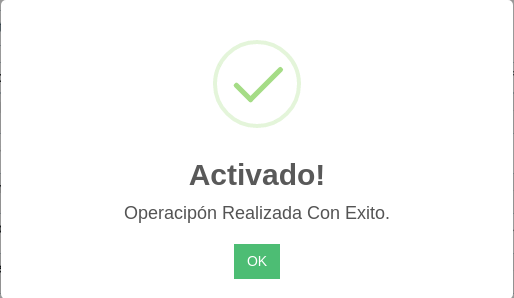
\includegraphics[scale=.5]{Pantallas/OperacionExitosa}
		\caption{MSG0: Operación exitosa}
	\end{center}
\end{figure}



\begin{figure}[htbp!]
	\begin{center}
		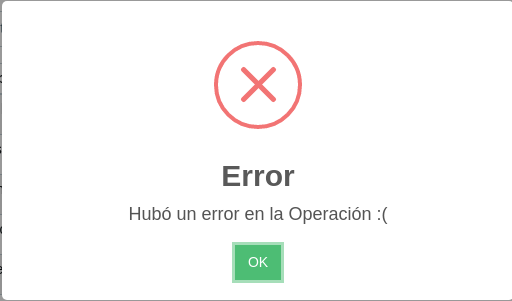
\includegraphics[scale=.5]{Pantallas/ErrorOperacion}
		\caption{MSG1: Error en la Operación}
	\end{center}
\end{figure}


\begin{figure}[htbp!]
	\begin{center}
		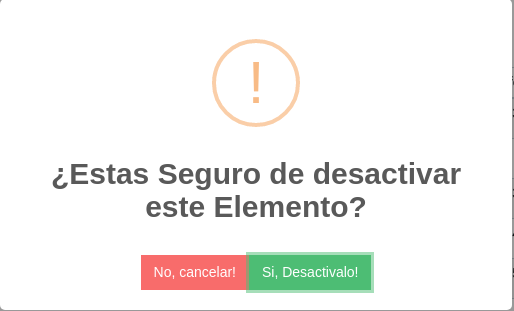
\includegraphics[scale=.5]{Pantallas/ConfirmacionDesactivar}
		\caption{MSG2: Confirmación de desactivar}
	\end{center}
\end{figure}

\begin{figure}[htbp!]
	\begin{center}
		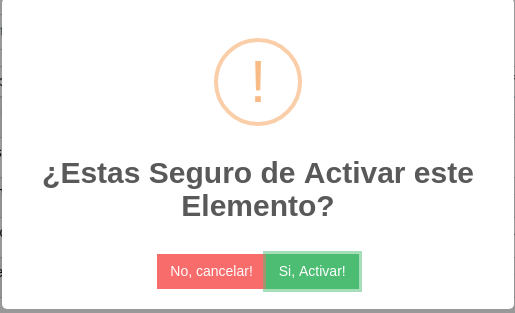
\includegraphics[scale=.5]{Pantallas/ConfirmacionActivar}
		\caption{MSG3: Confirmación de activar}
	\end{center}
\end{figure}

\begin{figure}[htbp!]
	\begin{center}
		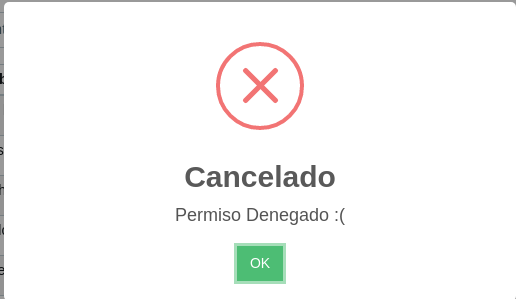
\includegraphics[scale=.5]{Pantallas/PermisoDenegado}
		\caption{MSG4: Permiso Denegado}
	\end{center}
\end{figure}


\begin{figure}[htbp!]
	\begin{center}
		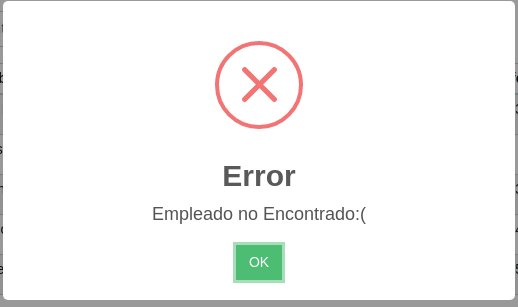
\includegraphics[scale=.5]{Pantallas/empleadoNoEncontrado}
		\caption{MSG5: Empleado No encontrado}
	\end{center}
\end{figure}

\begin{figure}[htbp!]
	\begin{center}
		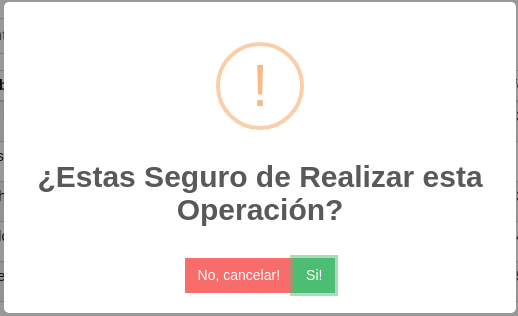
\includegraphics[scale=.5]{Pantallas/ConfirmacionOperacion}
		\caption{MSG6: Confirmar Operación}
	\end{center}
\end{figure}